\documentclass[12pt]{article}

\usepackage{graphicx}
\usepackage[rightcaption]{sidecap}

\title{RGB Image of Jupiter}
\date{2016 April 12}
\author{Brendon Walter}

\begin{document}
	\maketitle
	
	\section{Abstract}
	
	Two images of Jupiter were created using 9 total images with 3 images each taken in R, G, and B filters. Color processing and image alignment was done in AstroImageJ. In the final images, two main dark stripes can be seen on Jupiter as well as some lighter stripes. Additionally, the four Galilean moons can be seen, with thee of them on one side and the fourth one on the other. I created two images using two different methods - the first method created a clearer picture overall especially of the planet while second method resulted in a fuzzy image of Jupiter and with faint moons.
	
	\section{Jupiter}
	Jupiter, the fifth closest planet to the sun, is the most massive planet in our solar system with a mass that is 2.5 times the mass of all other planets in the solar system combined. [1] It is 318 times as massive as the Earth alone, although roughly 1,300 Earths would fit inside Jupiter due to its low density. [1] Jupiter's atmosphere resembles the sun in many ways [2] - both are almost entirely made up of hydrogen and helium (and only trace amounts of other elements), with hydrogen making up around three quarters of the total mass of both the sun and Jupiter. [1][3]
	\\\\
	The planet has at least 63 moons, the four largest of which - Io, Europa, Ganymede, and Callisto - were discovered by Galileo Galilei in the 1600s. [4]
	\\\\
	Several stripes, some of them dark and others lighter in color, can be seen on the planet. These stripes are caused by strong, 400 mph winds moving the gas in alternating directions in the atmosphere. [4]
	
	\section{Imaging}
	The final RGB images of Jupiter were created from 9 total images, with 3 images per filter. They were taken on April 6, 2016 starting at 00:51 and ending at 00:57 UT.
	\\\\
	Each image had an exposure time of 0.05 seconds so that each image would have a maximum count of 50,000 out of the 64,000 counts possible.
	\\\\
	These were taken with an SBIG STL-11000 3 CCD Camera mounted on a Optical Guidance Systems Ritchey-Chrétien 16 inch telescope in Bennington, Vermont.
	
	\section{Image Processing and Coloring}
	Color processing was done in AstroImageJ. I created a master flat for each filter (with 4 images per filter), where the flats were twilight sky flats taken the same night of observing. However, I believe most of these flats were too dim (less than 30,000 counts maximum for each image whereas I was aiming for 50,000 or so max) so it's questionable how useful they really are. Despite this, they were used anyway as it was assumed that poor flat correction was better than none. Dark and bias correction was done automatically by Maxim 5 when the images were taken.
	\\\\
	The corrected images were aligned in AstroImageJ by putting apertures around the four moons of Jupiter. Once aligned, they were stacked by filter using the Z Project stacking option, with the Project Type being set to Median. The images were then made into an RGB composite image.
	
		\begin{figure}
			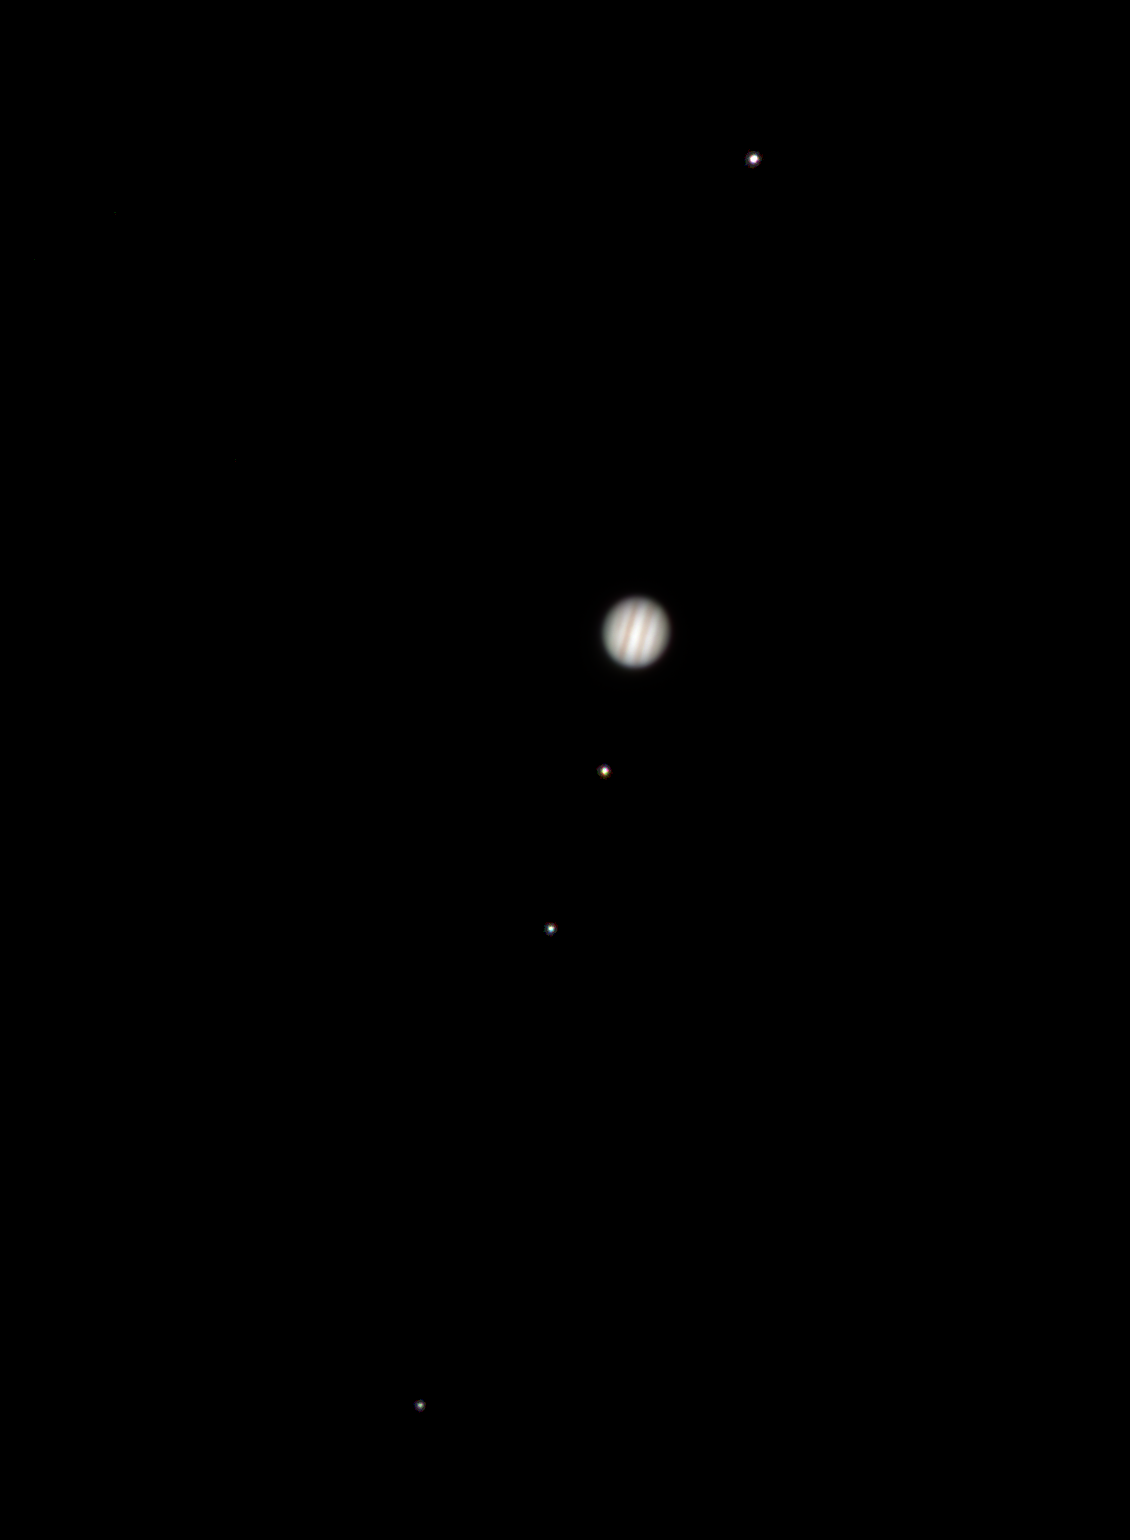
\includegraphics[height=500px]{./images/jupiter_moons_color_cropped}
			\caption{RGB Image of Jupiter created by layering two images, one of which highlighted the stripes of jupiter and the other which highlighted the moons.}
		\end{figure}
	
		\begin{figure}
			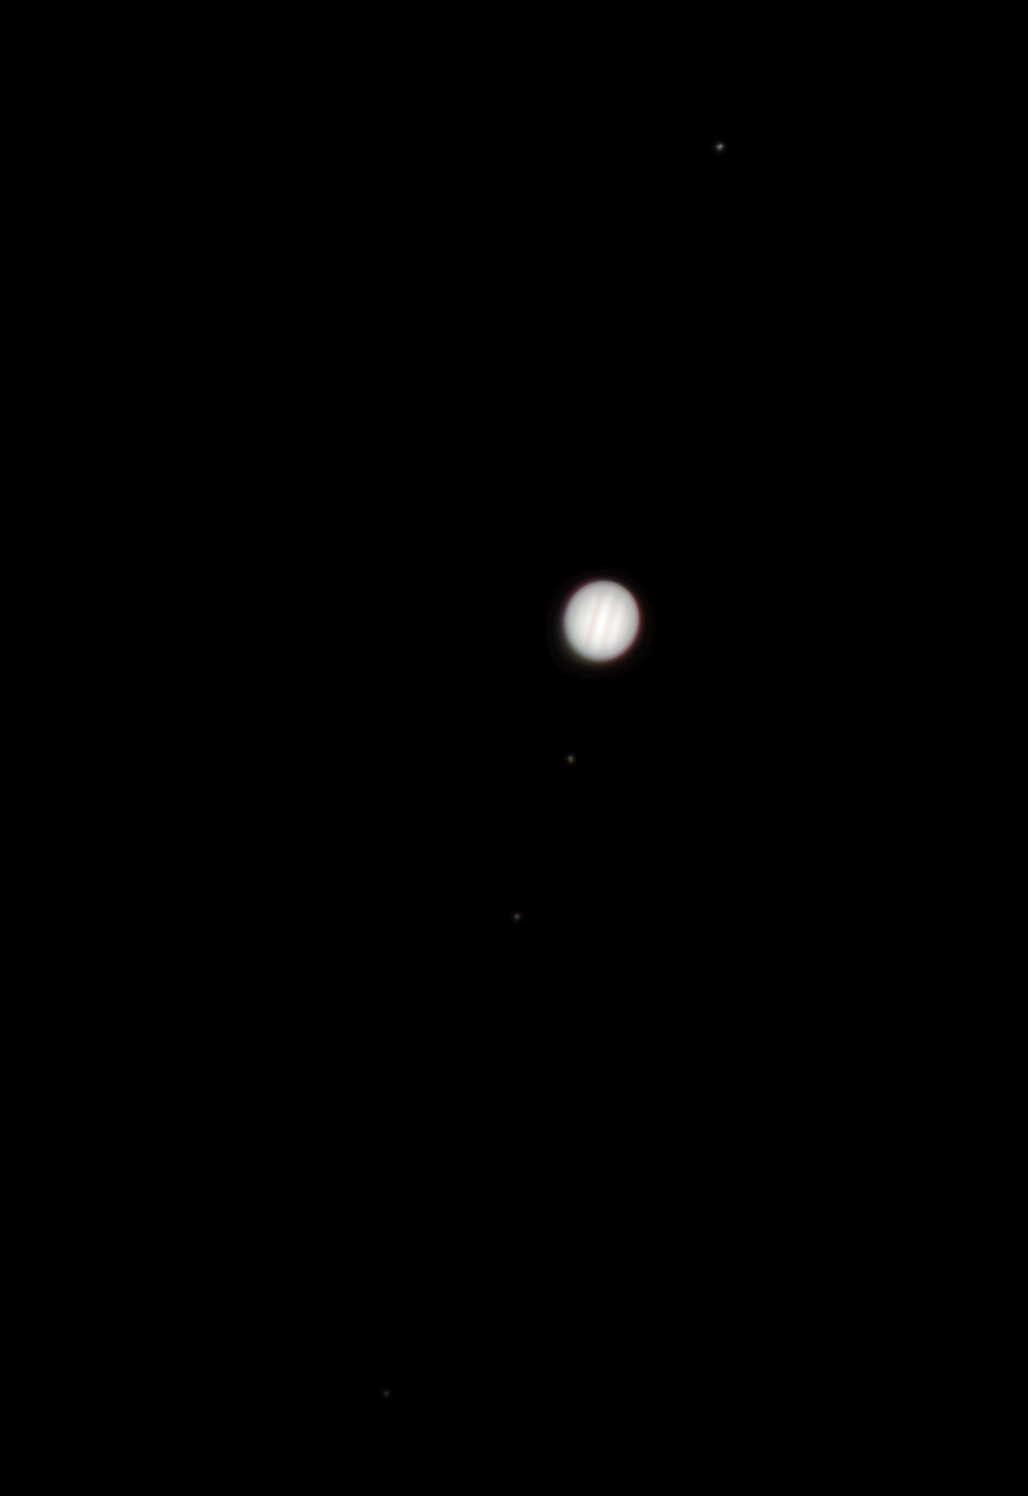
\includegraphics[height=500px]{./images/jupiter_curves_cropped}
			\caption{RGB Image of Jupiter and its moons using color curves in GIMP}
		\end{figure}
	
	\section{Results \& Discussion}
	Two dark stripes can be seen on Jupiter, as well as some lighter stripes. Additionally, the four Galilean moons can be seen, with thee of them on one side and the fourth one on the other. Creating an image that highlighted both the stripes and the moons proved to be difficult, as the moons are very faint and Jupiter is very bright. I used two different methods to create an image that showed both attributes:
	\begin{enumerate}
		\item I created two images, one in which the stripes were clear and the other in which the moons were visible. I layered the two images using GIMP and cut Jupiter out in the latter image, making it so the clearer image of the planet replaced the washed out one.  [Fig. 1]
		\item Using color curves in GIMP, I adjusted the image in which the stripes were visible until the moons were visible as well. [Fig. 2]
	\end{enumerate}
	The first method created a clearer image - the detail of the planet itself is crisp, each moon is bright and obvious, and slight differences in color for each moon can be seen as well. The second method created a fuzzy image of Jupiter and with faint moons.
	\\\\
	One thing to note is the size difference of the planet in each photo - in comparison to the moons, Jupiter appears to be much larger in the second image. Adjusting the curve changed the size of the planet, with a more washed out image being bigger and a clearer one being smaller.

	\section{Citations}
		\begin{enumerate}
			\item Williams, Matt. \emph{The Gas Giant Jupiter}. Universe Today. N.p., 25 Aug. 2015. Web. 12 Apr. 2016.
			\item \emph{Jupiter, Jupiter Information, Facts, News, Photos}. National Geographic. N.p., n.d. Web. 12 Apr. 2016.
			\item \emph{What Is Our Sun Made Of?} Space.com. N.p., 1 Mar. 2012. Web. 12 Apr. 2016.
			\item Choi, Charles Q. \emph{Planet Jupiter: Facts About Its Size, Moons and Red Spot}. Space.com. N.p., 14 Nov. 2014. Web. 12 Apr. 2016.
		\end{enumerate}
		
\end{document}